\documentclass{article}
\usepackage[utf8]{inputenc}
\usepackage{geometry}
 \geometry{
 a4paper,
 total={170mm,257mm},
 left=20mm,
 top=20mm,
 }
\usepackage{tikz}\usetikzlibrary{automata, positioning, arrows}

\title{ COMP 330 Winter 2021 \\ Assignment 1}
\author{Belle Pan 260839939}
\date{21st January 2021}

\usepackage{natbib}
\usepackage{graphicx}

\begin{document}

\maketitle

\noindent \textbf{Solution 1. 
\\Given a finite alphabet \(\Sigma\) and let \(\emptyset \neq L \subseteq \Sigma ^*\). 
We define the following relation \(R\) on words from \(\Sigma ^*\): 
\(\forall x, y \in \Sigma ^*, xRy\) if \(\forall z \in \Sigma^*, xz \in L\) iff \(yz \in L\).
Prove that this is an equivalence relation.}
\\
\\To prove this is an equivalence relation, we must check if it fulfills the three properties of an equivalence relation: reflexitivity, symmetry, and transitivity.
\begin{enumerate}
    \item Reflexitivity: \(\forall x \in \Sigma ^ *,\) \(xRx\)
    \begin{itemize}
        \item In this case, we see that \(\forall z \in \Sigma^*,\) \(xz \in L\) iff \(xz \in L\).
        \item This case holds (i.e. is true) because \(xz \in L\) is on both sides of the iff statement.
    \end{itemize}
    \item Symmetry: \(\forall x,y \in \Sigma ^ *,\) \(xRy \Longrightarrow yRx\)
    \begin{itemize}
        \item In this case, we see that \(\forall z \in \Sigma^*,\) \(xz \in L\) iff \(yz \in L\) implies that \(\forall z \in \Sigma^*,\) \(yz \in L\) iff \(xz \in L\).
        \item This is clearly true, as the iff statement may be reversed.
    \end{itemize}
    \item Transitivity: \(\forall x,y,z \in \Sigma ^ *,\)
    \\1) If \(\forall w \in \Sigma^*,\) \(xw \in L\) iff \(yw \in L\)
    \\2) And \(\forall w \in \Sigma^*,\) \(yw \in L\) iff \(zw \in L\)
    \\3) Then \(\forall w \in \Sigma^*,\) \(xw \in L\) iff \(zw \in L\)
    \begin{itemize}
        \item First, supposing \(w\in \Sigma ^ *\) and supposing \(xw \in L\), we know that \(yw\in L\) by 1).
        \item Knowing that \(yw\in L\), we also gather that \(zw\in L\) by 2). We also know that if \(zw\in L\), then \(yw\in L\) (the iff statement implies both ways!).
        \item Hence, we can conclude using 3) that if \(zw\in L\) then \(xw \in L\).
    \end{itemize}
\end{enumerate}
All properties hold; therefore, \(R\) is an equivalence relation.
\\
\\\noindent \textbf{Solution 2. 
\\Consider, pairs of natural numbers \( \langle m, n \rangle\) where \(m, n\in N\). We order them by the relation \( \lange m, n\rangle \sqsubseteq \langle m', n'\rangle\) if \(m < m'\) or \((m = m') ^ \land n \leq n'\), where \(\leq\) is the usual numerical order. Prove that the relation \(\sqsubseteq\) is a partial order.}
\\
\\To prove that \(\sqsubseteq\) is a partial order, we must check if it fulfills the three properties of a partial order: reflexitivity, antisymmetry, and transitivity.
\begin{enumerate}
    \item Reflexitivity: \(\forall x \in \Sigma ^ *,\) \(xRx\)
    \begin{itemize}
        \item \( \langle m, n \rangle\) compared with itself yields \(m=m\), and we also see that \(n \leq n\).
        \item Therefore, \( \langle m, n \rangle \sqsubseteq \langle m, n \rangle\) (clearly reflexive).
    \end{itemize}
    \item Antisymmetry: \(\forall x,y \in \Sigma ^ *,\) if \(xRy\) and \(yRx\) \(\Longrightarrow x=y\)
    \begin{itemize}
        \item Suppose that \( \langle m_1, n_1 \rangle \sqsubseteq \langle m_2, n_2 \rangle\) and \( \langle m_2, n_2 \rangle \sqsubseteq \langle m_1, n_1 \rangle\) both hold.
        \item If \(m_1>m_2\), then this contradicts the first statement in which  \( \langle m_1, n_1 \rangle \sqsubseteq \langle m_2, n_2 \rangle\) holds. 
        \item Similarly, if \(m_1<m_2\), then this contradicts the statement in which \( \langle m_2, n_2 \rangle \sqsubseteq \langle m_1, n_1 \rangle\) holds.
        \item Therefore, \(m_1\) must be equal to \(m_2\) if both statements hold.
        \item Now, we know that these statements must also be true: \(n_1\leq n_2\), and \(n_2\leq n_1\).
        \item The only way this is possible is if \(n_1 = n_2\).
        \item Thus, we can conclude that \( \langle m_1, n_1 \rangle\) and \( \langle m_2, n_2 \rangle\) are equal.
    \end{itemize}
    \item Transitivity: \(\forall x,y,z \in \Sigma ^ *,\)
    \\1) If \(\forall w \in \Sigma^*,\) \(xw \in L\) iff \(yw \in L\)
    \\2) And \(\forall w \in \Sigma^*,\) \(yw \in L\) iff \(zw \in L\)
    \\3) Then \(\forall w \in \Sigma^*,\) \(xw \in L\) iff \(zw \in L\)
    \begin{itemize}
        \item In this case, we must show that \( \langle m_1, n_1 \rangle \sqsubseteq \langle m_3, n_3 \rangle\) given that \( \langle m_1, n_1 \rangle \sqsubseteq \langle m_2, n_2 \rangle\) and \( \langle m_2, n_2 \rangle \sqsubseteq \langle m_3, n_3 \rangle\).
        \item This leads us to the following cases:
        \begin{itemize}
            \item If \(m_1<m_2\) and \(m_2<m_3\), then \(m_1<m_3 \Longrightarrow \langle m_1, n_1 \rangle \sqsubseteq \langle m_3, n_3 \rangle\).
            \item If \(m_1<m_2\) and \(m_2=m_3\), then \(m_1<m_3 \Longrightarrow \langle m_1, n_1 \rangle \sqsubseteq \langle m_3, n_3 \rangle\).
            \item If \(m_1=m_2\) and \(m_2=m_3\), then \(m_1<m_3 \Longrightarrow \langle m_1, n_1 \rangle \sqsubseteq \langle m_3, n_3 \rangle\).
            \item If \(m_1=m_2\), \(m_2=m_3\), \(n_1 \leq n_2\), and \(n_2 \leq n_3\), then we must have \(m_1 = m_3\) and \(n_1 \leq n_3\). As both equality and \(\leq\) are transitive, this implies \(\langle m_1, n_1 \rangle \sqsubseteq \langle m_3, n_3 \rangle\).
        \end{itemize}
    \end{itemize}
\end{enumerate}
All properties hold; therefore, \(\sqsubseteq\) is a partial order.
\\
\\\noindent \textbf{Solution 3. 
\\Give deterministic finite automata accepting the following languages over
the alphabet \( \{0,1\}\).
\begin{enumerate}
    \item The set of all words ending in 00.
    \item The set of all words ending in 00 or 11.
    \item The set of all words such that the second last element is a 1.
\end{enumerate} }

\begin{figure}[ht]
   \centering
    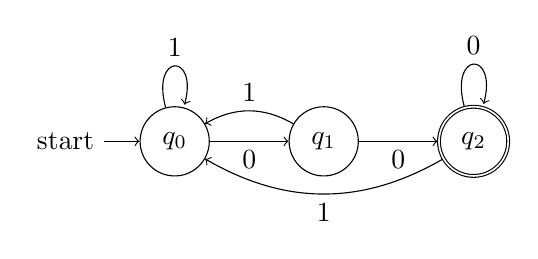
\begin{tikzpicture}
        \node[state,initial](q_0) {$q_0$};
        \node[state] (q_1) [right=of q_0] {$q_1$};
        \node[state,accepting] (q_2) [right=of q_1] {$q_2$};
        \path[->] 
                (q_0) edge node [below] {0} (q_1)
                    edge [loop above] node {1} ()
                (q_1) edge node [below] {0} (q_2)
                    edge [bend right] node [above] {1} (q_0)
                (q_2) edge [bend left] node [below] {1} (q_0)
                    edge [loop above] node {0} ();
    \end{tikzpicture}
    \caption{Deterministic finite automata accepting the set of all words ending in 00.}
    \label{fig:my_label}
\end{figure}


\begin{figure}[ht]
   \centering
    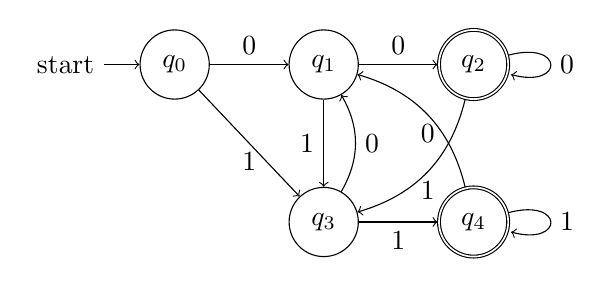
\begin{tikzpicture}
        \node[state,initial](q_0) {$q_0$};
        \node[state] (q_1) [right=of q_0] {$q_1$};
        \node[state,accepting] (q_2) [right=of q_1] {$q_2$};
        \node[state] (q_3) [below of= q_1, yshift=-1cm] {$q_3$};
        \node[state, accepting] (q_4) [below of= q_2, yshift=-1cm] {$q_4$};
        \path[->] 
                (q_0) edge node [above] {0} (q_1)
                    edge node [below] {1} (q_3)
                (q_1) edge node [above] {0} (q_2)
                    edge node [left] {1} (q_3)
                (q_2) edge [bend left] node [below] {1} (q_3)
                    edge [loop right] node {0} ()
                (q_3) edge [bend right] node [right] {0} (q_1)
                    edge node [below] {1} (q_4)
                (q_4) edge [bend right] node [below] {0} (q_1)
                    edge [loop right] node {1} ();
    \end{tikzpicture}
    \caption{Deterministic finite automata accepting the set of all words ending in 00 or 11.}
    \label{fig:my_label}
\end{figure}

\begin{figure}[ht]
   \centering
    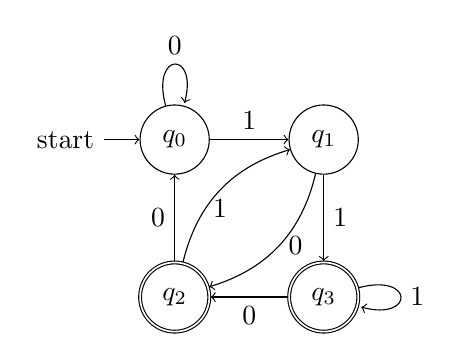
\begin{tikzpicture}
        \node[state,initial](q_0) {$q_0$};
        \node[state] (q_1) [right=of q_0] {$q_1$};
        \node[state,accepting] (q_2) [below of= q_0, yshift=-1cm] {$q_2$};
        \node[state, accepting] (q_3) [below of= q_1, yshift=-1cm] {$q_3$};
        \path[->] 
                (q_0) edge node [above] {1} (q_1)
                    edge [loop above] node {0} ()
                (q_1) edge [bend left] node [right] {0} (q_2)
                    edge node [right] {1} (q_3)
                (q_2) edge [bend left] node [below] {1} (q_1)
                edge node [left] {0} (q_0)
                (q_3) edge [loop right] node [right] {1} ()
                edge node [below] {0} (q_2);
    \end{tikzpicture}
    \caption{Deterministic finite automata accepting the set of all words such that the second last element is a 1.}
    \label{fig:my_label}
\end{figure}

\noindent \textbf{Solution 4. 
\\Suppose that \(L\) is a language accepted by a DFA (i.e. a regular language). Show that the following language is also regular: lefthalf\((L) := \{w_1 | \exists w_2 \in \Signma^*\) such that \(w_1 w_2 \in L\) and \(|w_1|=|w_2|\}\).}
\\
\\Let \(L\) be defined as \((Q, q_0,\delta, F)\). Let us then define a new NFA denoted \(L'\) as \((Q', Q_0', \Delta, F')\), where
    \begin{itemize}
        \item\(Q' = Q \times Q\), i.e. the states in \(L'\) are pairs of states from the machine of \(L\)
        \item \(Q_0' = \{(q_0,f)|f \in F\}\)
        \item \(\Delta((s,t),a) = \{(\delta(s,a),t')|t=\delta(t',b)\) for some \(b\in \Sigma\}\)
        \item \(F'=\{(s,s)|s\in Q\}\)
    \end{itemize}
\\We may note a couple of characteristics of \(L'\):
\begin{itemize}
    \item Given a word \(w\), the states in \(L'\) keep track of how the machine for \(L\) processes \(w\) via the first element in the pair; the second element of the pair keeps track of all the possible paths possible via processing \(w\) letter by letter by traversing through the states of the machine for \(L\) starting from an accept state.
    \item If \(L'\) finishes processing \(w\) (i.e. it reaches the end of \(w\)) and ends at the state \((q_n,q_n)\), the machine for \(L\) will have also ended in the state \(q_n\) after processing \(w\).
\end{itemize}
Looking at the second element of the pair of states in \(L'\), we observe that it took \(|w|\) transitions from an accept state to reach \(q_n\). 
\begin{itemize}
    \item This leads us to the understanding that there must be a path in the machine of \(L\) that starts at \(q_n\) and ends in an accept state.
    \item Therefore, there must exist another word \(w'\) of which, when read after \(w\) by the machine of \(L\), would reach an accept state. I.e. If the machine reads \(ww'\), reading \(w\) would take us from the start state to \(q_n\) and reading \(w'\) after it would take us from \(q_n\) to an accept state.
\end{itemize}
This concludes that \(ww' \in L\) and \(w\) would only be accepted by \(L'\) if \(w \in\) lefthalf\((L)\). Hence, lefthalf\((L)\) must be a regular language. 
\\\\
\noindent \textbf{Solution 5. 
\begin{enumerate}
    \item Give a deterministic finite automaton accepting the following language over the alphabet \(\{0,1\}\): The set of all words containing \(100\) or \(110\).
    \item Show that any DFA for recognizing this language must have at least \(5\) states.
\end{enumerate} }

\begin{figure}[ht]
   \centering
    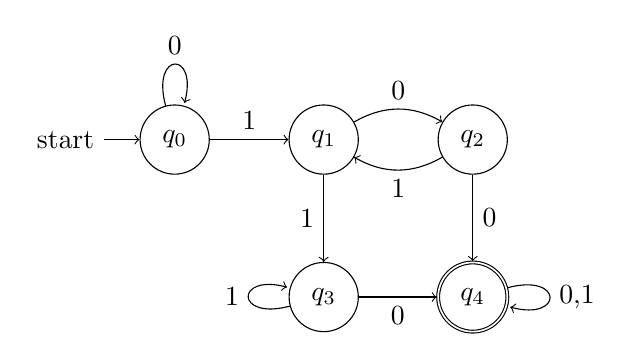
\begin{tikzpicture}
        \node[state,initial](q_0) {$q_0$};
        \node[state] (q_1) [right=of q_0] {$q_1$};
        \node[state] (q_2) [right=of q_1] {$q_2$};
        \node[state] (q_3) [below of= q_1, yshift=-1cm] {$q_3$};
        \node[state, accepting] (q_4) [below of= q_2, yshift=-1cm] {$q_4$};
        \path[->] 
                (q_0) edge node [above] {1} (q_1)
                    edge [loop above] node {0} ()
                (q_1) edge [bend left] node [above] {0} (q_2)
                    edge node [left] {1} (q_3)
                (q_2) edge [bend left] node [below] {1} (q_1)
                    edge node [right] {0} (q_4)
                (q_3) edge [loop left] node [left] {1} ()
                    edge node [below] {0} (q_4)
                (q_4) edge [loop right] node [right] {0,1} ();
    \end{tikzpicture}
    \caption{Deterministic finite automata accepting the set of all words containing \(100\) or \(110\) over the alphabet \(\{0,1\}\).}
    \label{fig:my_label}
\end{figure}
\noindent This DFA may receive five different types of words and end up in five states:
\begin{enumerate}
    \item \(\varepsilon\), which ends up in a state we denote \(s_0\)
    \item \(1\), which leads to a state we denote \(s_1\) from the start state
    \item \(10\), which leads to a state we denote \(s_2\) from the start state
    \item \(11\), which leads to a state we denote \(s_3\) from the start state
    \item \(110\), which leads to a state we denote \(s_4\) from the start state
\end{enumerate}

\noindent We check to see if any of the states stated above are redundant (i.e. if two of the above words leads to the same state):
\begin{itemize}
    \item \(s_4\) must be different than all the other states, as the DFA accepts \(110\) and none of the other words listed above without some form of modification.
    \item If \(s_0 = s_1\), this means that \(\varepsilon\) and \(1\) must reach the same state; however, if this were the case, \(\varepsilon \cdot 10\) and \(1 \cdot 10\) should both be accepted by the DFA. \(10\) is not accepted by the DFA, and thus \(s_0\) and \( s_1\) must be distinct.
    \item If \(s_0 = s_2\), this means that \(\varepsilon\) and \(10\) must reach the same state; however, if this were the case, \(\varepsilon \cdot 0\) and \(10 \cdot 0\) should both be accepted by the DFA. \(0\) is not accepted by the DFA, and thus \(s_0\) and \( s_2\) must be distinct.
    \item If \(s_0 = s_3\), this means that \(\varepsilon\) and \(11\) must reach the same state; however, if this were the case, \(\varepsilon \cdot 0\) and \(11 \cdot 0\) should both be accepted by the DFA. \(0\) is not accepted by the DFA, and thus \(s_0\) and \( s_3\) must be distinct.
    \item If \(s_1 = s_2\), this means that \(1\) and \(10\) must reach the same state; however, if this were the case, \(1 \cdot 0\) and \(10 \cdot 0\) should both be accepted by the DFA. \(10\) is not accepted by the DFA, and thus \(s_1\) and \( s_2\) must be distinct.
    \item If \(s_1 = s_3\), this means that \(1\) and \(11\) must reach the same state; however, if this were the case, \(1 \cdot 0\) and \(11 \cdot 0\) should both be accepted by the DFA. \(0\) is not accepted by the DFA, and thus \(s_1\) and \( s_3\) must be distinct.
    \item If \(s_2 = s_3\), this means that \(10\) and \(11\) must reach the same state; however, if this were the case, \(10 \cdot 10\) and \(11 \cdot 10\) should both be accepted by the DFA. \(1010\) is not accepted by the DFA, and thus \(s_2\) and \( s_3\) must be distinct.
\end{itemize}
Therefore, there must be five distinct states in this DFA for it to function properly.



\end{document}
